\documentclass[11pt,a4paper,titlepage]{article}

%%%%%%%%%
%%usees%%
%%%%%%%%%
\usepackage[utf8]{inputenc}
%\usepackage[ngerman]{babel}
\usepackage{setspace}
\usepackage{graphicx}
\usepackage{amssymb} 
\usepackage{amsmath}
\usepackage{mathtools}
\usepackage{footnote}
\usepackage{caption}
\usepackage{color}
\usepackage{hyperref}
\usepackage{cite}




%%%%%%%%%
%%Title%%
%%%%%%%%%
\author{Frederik Zwilling 304314}
\title{Proposal:\\ Bachelorthesis Simulation LLSF with Gazebo}
\begin{document}
\maketitle
%\thispagestyle{empty}
%\tableofcontents
%\newpage
%\onehalfspace

%%%%%%%%%
%%Text%%
%%%%%%%%
\abstract{Short description}
\section{Introduction}
Autonomous robots are about to play an important role in the future of logistics. They will be able to save time and cost in the industrial production process and boost the economy. Especially multi-robot-systems play an important role in this context. They are able to do distributed work, are efficient if they work together and are reliable regarding downtime of single robots. Though, the development of these logistic robots can be difficult because the robots have to handle many complex tasks. They have to detect objects, localize themselves, make a plan of what to do in which order, coordinate with other robots, optimize the work flow, be save for humans and hardware at every time and much more.\\
The key to effective and time saving development of reliable software for robots is simulation. Simulation makes it possible to virtually test written code fast in different scenarios.This leads to better quality of the software and better performance of the robot. By simulating the behavior of a robot much time can be saved because there is no real robot which has to be set up and the simulation can quickly change between different scenarios. Furthermore it is possible to speed the simulation up or run multiple simulations at once. Simulation also makes testing possible if no real robot is available and can be easily used to compare different versions of the software. For example this can be useful to find unknown parameters like thresholds.\\
The proposed bachelor-thesis will work on this area and will develop a simulation environment for the \textit{Logistic League Sponsored by Festo} (LLSF) with the robot software framework \textit{fawkes}~\footnote{\url{www.fawkesrobotics.org}} and the open source simulator \textit{Gazebo}. The emphasis will be the multi-robot aspect of the simulation.
\subsection{Logistic League Sponsored by Festo}
The Logistic League Sponsored by Festo is part of the \textit{RoboCup
}, an international robotics competition~\footnote{\url{http://www.robocup.org/}}. LLSF aims to catalyze scientific work on autonomous solutions for logistics. The participants should find new approaches and improve already existing ones to optimize material and information flow in the industrial production. LLFS is realized in a fictional production hall. 
\begin{figure}
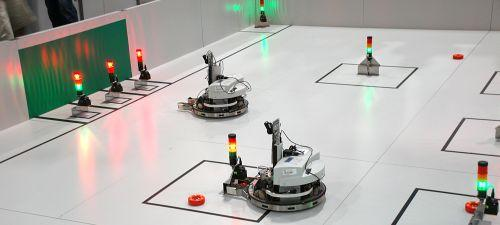
\includegraphics[scale=0.7]{pics/llsf1}
\label{Figure 1}
\caption{A half of the LLSF field.  \textcolor{red}{refferenz schrecklich~\cite{LLSFGermanOpen}}}
\end{figure}
Figure 1 shows this hall and the basic elements. The Robots are Robotinos by Festo~\cite{Robotino}. They hold omni-directional wheels, a showel to move pucks and other sensors added by the participants. The orange pucks represent resouces and products. They are equiped with a RFID-chip which stores the type of the puck. The lamps on the field are the machines. They use RFID to convert recourses into producs and trash. There are different types of machines. They can produce different product-types, produce intermediate products, recycle trash or are used for delivery. The traffic-light on top of the machines indicates the machine-status. Beside these visual elements there is also a refbox which automatically communicates with the robots during the game. The refbox provides the current phase and tasks of the game.
\subsection{Fawkes}
Fawkes is an open source robot software framework developed by the Knowledge-basede Systems Group~\footnote{\url{http://www.kbsg.rwth-aachen.de/}} at RWTH Aachen University. It is written for Linux and follows a component-based software design~\cite{FawkesDesign}. It provides an infrastructure to load and unload binary components, implemented as plugins, at runtime and a blackboard for communication between the plugins. A plugin can access the blackboard via interfaces. Because of this design, Fawkes is very flexible and dynamic. The interchangeability of the plugins, which is caused by the well defined interfaces, makes hardware abstraction and reuse easy.\\
\subsection{Gazebo}
Gazebo is an open source multi-robot simulator~\cite{GazeboDesign}. It simulates the behavior of robots and other objects physically in a three dimensional world. The open source engine Ogre~\footnote{\url{http://www.ogre3d.org}} is used for the graphical presentation of the simulation. Physics are simulated with the Open Dynamics Engine~\footnote{\url{http://www.ode.org/}}. Gazebo was originally developed for outdoor applications and aims to simulate robots in a complex and realistic environment. Besides the physical simulation, it does this by generating data for different types of sensors. Gazebo can simulate laser range finders, cameras, sonar sensors, bumpers and more. This makes it able to do realistic and low level simulation. A simulation in Gazebo is made by creating robot and world models and developing Gazebo-plugins for behavior. These plugins can control objects in Gazebo and communicate with other software.
\subsection{Proposed Bachelor Thesis}
The primary goal of the proposed bachelor thesis is to develop a simulation environment in Fawkes for the LLSF competition with Gazebo. This will speed up and simplify many current and future developments. Some of the the current developments are a high level agent for the exploration phase of LLSF, a laser-cluster-detector that locates obstacles with a laser sensor and a map of the environment and a vision detector for different combinations of light signals including blinking lamps. All these can benefit from the simulation. The agent can easily be tested because its behavior is shown visual in realistic simulation. The current simulation for the high level agent is only text-based and does not simulate any actions on a lower level (e.g. all movement orders return that they succeeded after a few seconds). The laser-cluster-detector would benefit from the simulation because the laser data generated done by Gazebo is relatively realistic~\footnote{This has to be proven by the thesis, but it is intuitively right because laser sensors are quite accurate and a geometrical calculation by Gazebo is easy.} and it is possible to look at different situations much faster. Even the vision task can benefit from the simulation because the vision plugin can first be made working as a whole with simple images. The neccessary vision tuning can then be done as a second step with a already tested structure it is embedded in. Of course simulation never can completely substitute testing on the real robot, but it saves a lot of time. This has many causes. There is no need to get the real robot running which can take a lot of time in practise. The logic can be tested seperate from real world problems such as inaccuracy or badly synchronized clocks. An other advantage of the simulation is that ever the developers do not work on the same system. So there are no messed up configuration files and less problems with revision controlling.\\
Structural, the multi-robot simulation for LLSF will consist of Fawkes and Gazebo plugins and models for Gazebo. The interchangeability of plugins in Fawkes makes it possible that the simulation only needs to exchange the robot hardware plugins on the lowest level by robot simulation plugins. All plugins on upper levels do not need to be changed and can work in the simulation the same way as in reality. The models for Gazebo will represent all physical objects in the LLSF game (e.g. the Robotino and the Machines). The Gazebo plugins will control the behavior and sensing of all dynamic elements in the game (e.g. the Robotino and the refbox).\\
In the following the proposal will give an overview of the related work in section 2. This section will be divided in the context the thesis will be embedded in, other simulators and other multi-robot simulations. Section 3 will present the proposed work in detail with primary and further goals. Section 4 will give a schedule and in section 5 some methods of afterwards evaluation are proposed. The conclusion is found in section 6.


\section{Related Work}
\section{Detail}
\section{Timetable}
\section{Evaluation}
\section{Conclusion}

\bibliographystyle{plain}
\bibliography{references}

\end{document}
